\chapter{Summary and Future Directions}\label{chap:conclusion}

In this chapter, I summarize the main findings of this thesis briefly
and outline some future directions that are not direct extensions on the
works documented in previous chapters.

My work focuses on improving the RV precision of \het\ and \keck, with
the goal to improve the RV precision of \het\ to beyond 3 m/s and to
the level of \keck, around 1-2 m/s. The code I adopted for RV extraction
is the widely used CPS Doppler code written by Marcy, Butler, Johnson
et al. (Chapter~\ref{chap:doppler}). I examined the causes behind
\het's lower RV precision in comparison to \keck\ and came to the
conclusion that the gas in the HRS iodine cell was not at its
set-temperature of 70$\degree$C. However, the iodine atlas that was
used for modeling \het\ data for years was taken at an iodine gas
temperature of around 70$\degree$C. This discrepancy lead to the poor
goodness of fits for \het\ spectra and higher RV RMS. The other cause
is inaccurate IP modeling, where the current IP functions often have a
hard time to converge onto a good solution due to the inaccurate
iodine model, a lack of good initial guesses, and/or intrinsic
complexity with the IP function itself. I believe that a more robust
temperature control system and a (series of) validated FTS scan(s) for
the \het\ iodine cell, plus a good IP function, will improve the RV
precision of \het, including its archival data (Chapter~\ref{chap:het}).

My primary goal for improving \keck\ precision is to pin down the
causes for the RV systematic errors that manifest as correlations or
trends between RV and BC. I conclude that the leading cause is the
errors in \keck's deconvolved stellar spectral template (DSST), which
adds about 1 m/s to the error budget and is directly driving the RV-BC
correlation. There are also secondary causes being algorithmic errors
and telluric contamination, entering the error budget at 0.2-0.5 m/s
level. I believe that a better algorithm for generating DSST, proper
treatment for telluric contamination, and adoption for a more robust
algorithm will bring the RV precision of \keck\ to the next level
(Chapter~\ref{chap:keck}). 

I have also done some works in characterizing planetary orbits using
RV data. Most notably, I have published the {\tt BOOTTRAN} package,
which computes error bars for Keplerian fits via bootstrapping
(Chapter~\ref{chap:boottran}). We have discovered a new planet, HD
37605$c$, using \het\ data analyzed by the adopted CPS Doppler code
and also \keck\ RVs (Chapter~\ref{chap:planets}).

In the concluding sections of Chapter~\ref{chap:het} and
\ref{chap:keck}, we have summarized future works which are natural
next steps to improve the RV precision of \het\ and \keck. Beyond
these next steps, there are also other independent paths I plan to
take in continuing my journey in exoplanet discoveries using precise
Doppler spectroscopy.

First of all, I am constructing a new RV code in {\it Python}. The CPS
Doppler code is a great legacy code which works at 1-2 m/s level, but
it has many drawbacks: It is based on a simple home-constructed
Levenberg–-Marquardt least $\chi^2$ fitter (LM fitter) which has high
requirement on initial guesses for parameters and is terribly
inefficient and inadequate in exploring the $\chi^2$ space and finding
the true minimum. It also has many legacy house keeping parts and
complicated structures that makes it hard to upgrade, adopt for other
instruments, and add new modules and functions. The new code carries
on the valuable successful parts of the CPS code over, and more
importantly, built to be highly modular and thus easy to adopt for
other instruments or to plug in modern numerical and statistical
tools. It employs advanced statistical and numerical tools such as a
MCMC algorithm for Bayesian statistics and Gaussian processes
(Figure~\ref{fig:newrv2}), which will model the correlated noise
originated from a complex blaze function, normalization issues, CCD
effects, telluric line modeling residuals, imperfect deconvolved
stellar spectrum, and so on (see, e.g., \citealt{starfish} and Daniel
Foreman-Mackey's {\it george} package). The preliminary result from
this code (fitting for a spectral chunk) is shown in
Figure~\ref{conclusion:fig:mcmc}.


%----------------------------------------------------------------
% MCMC triangle plot for a Keck chunk fit
% plot from Jobs/plots/, made by newrv code and hand edited for 2015
% postdoc proposals
\begin{figure}
\centering
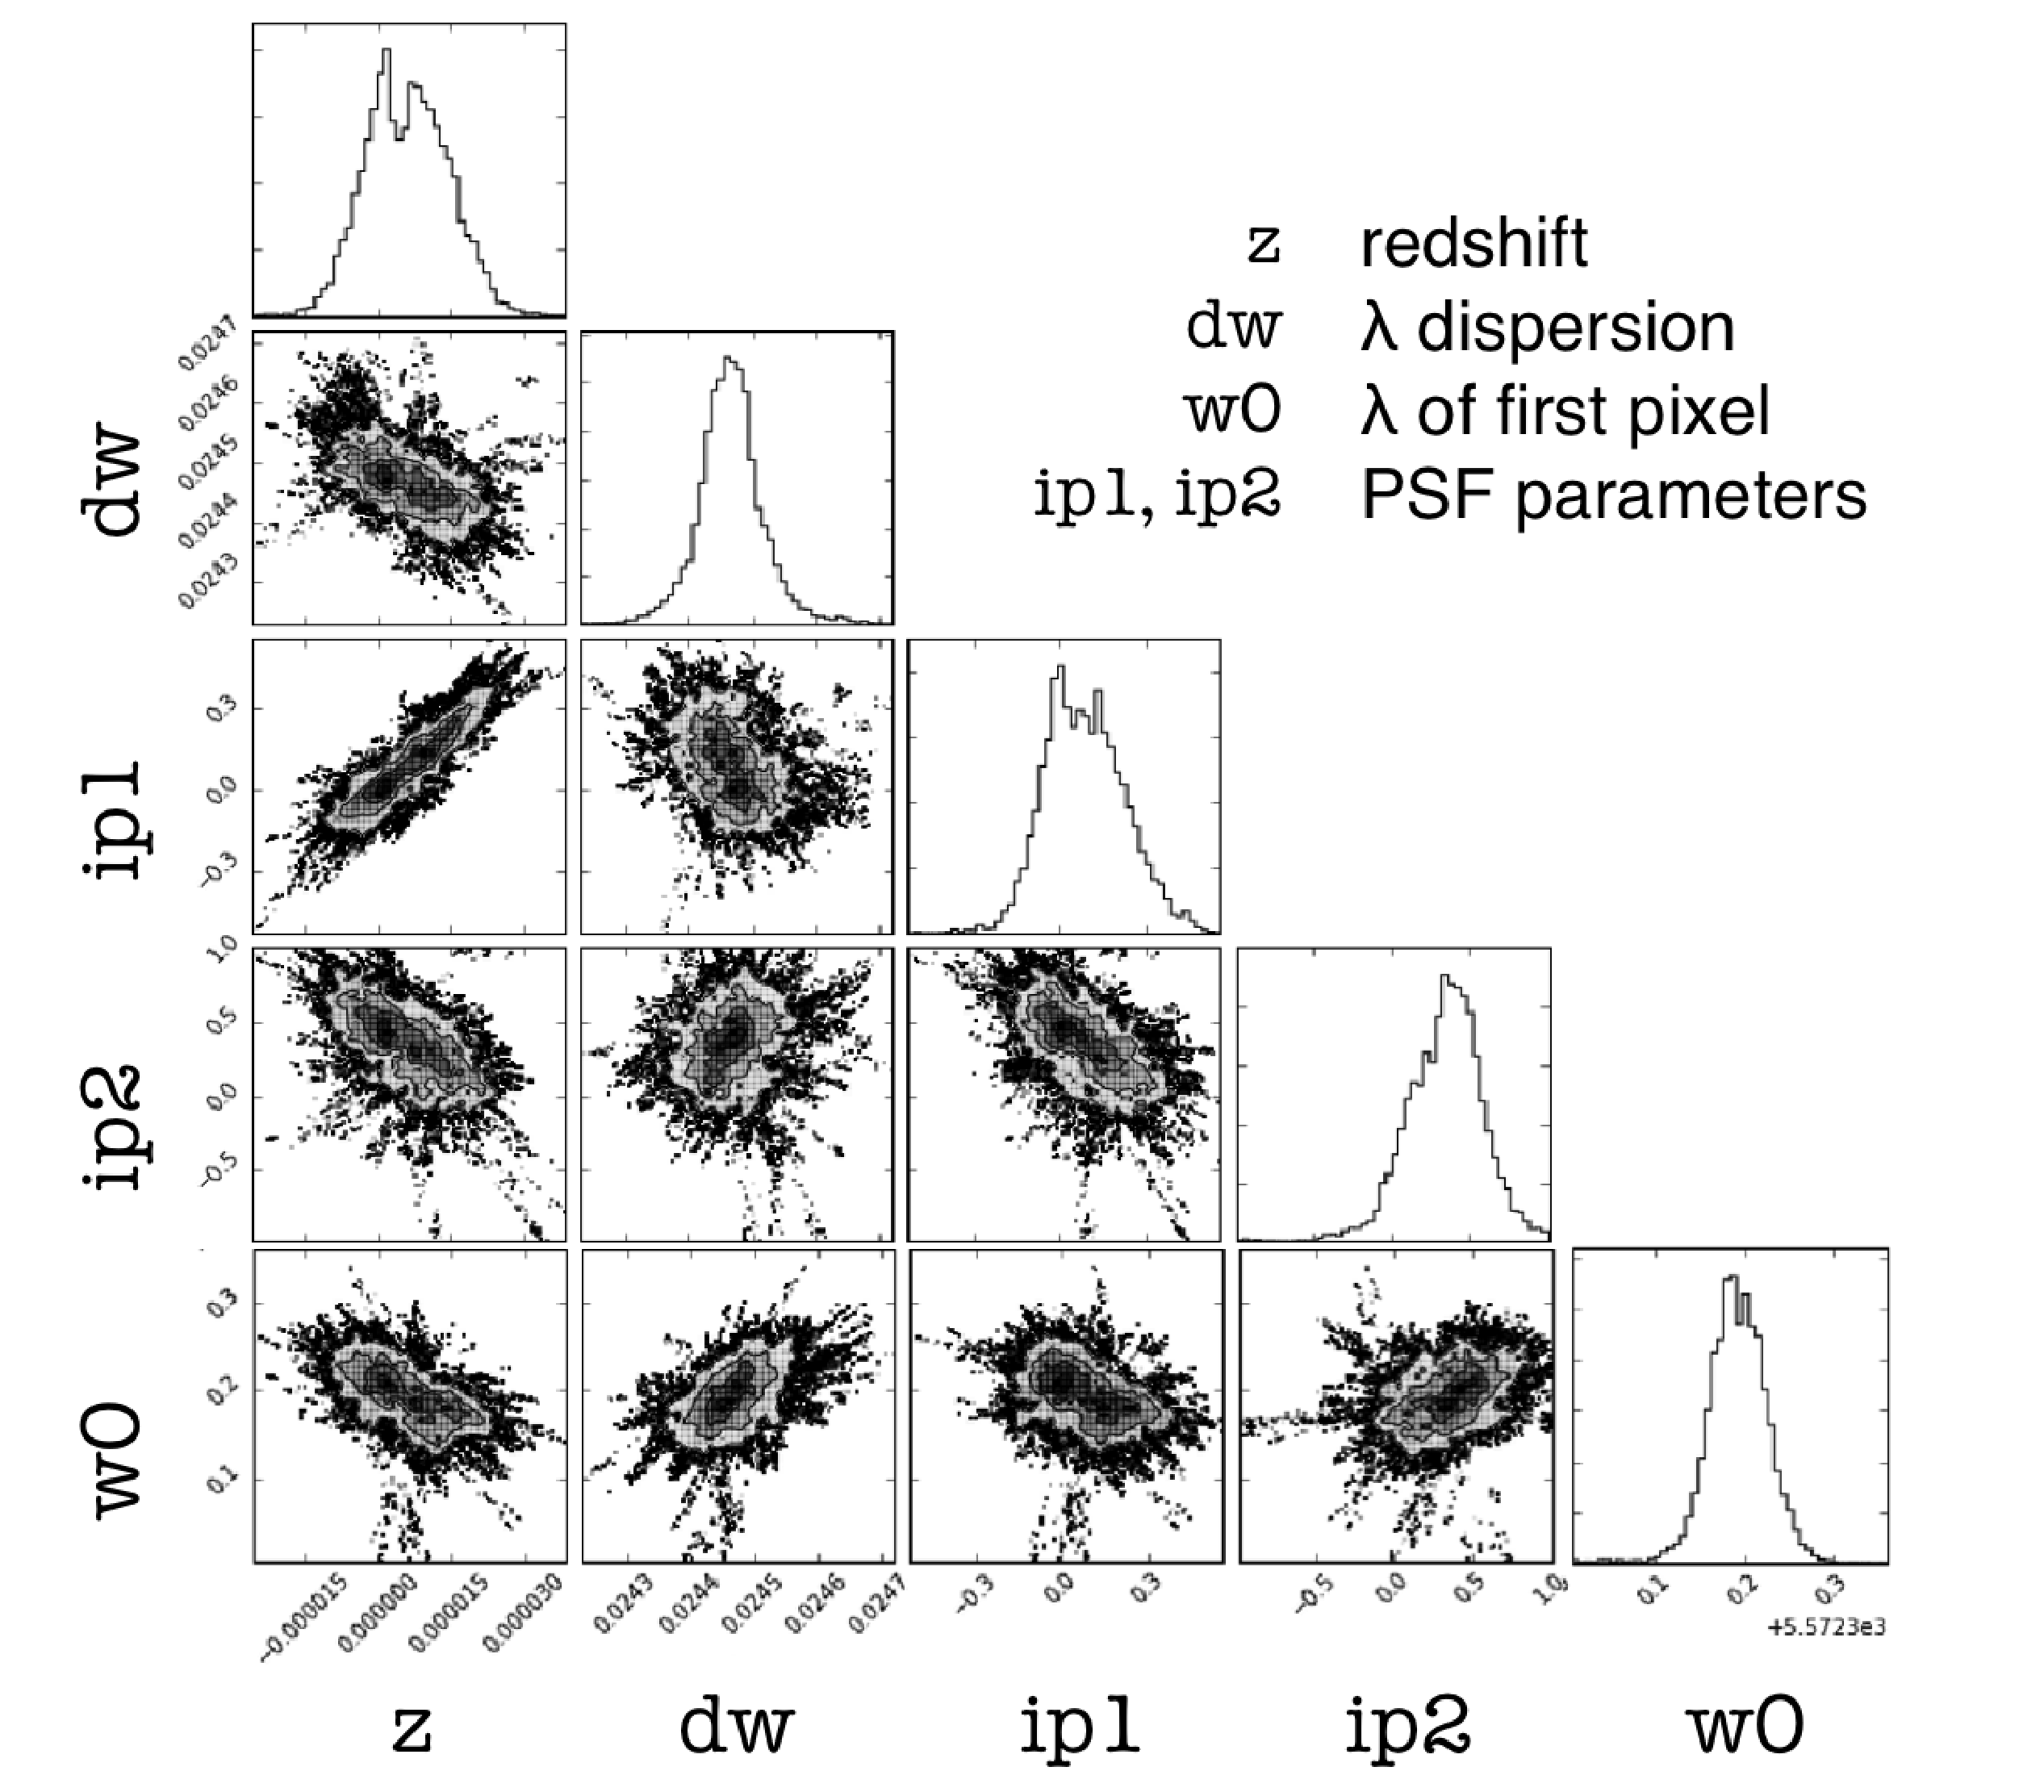
\includegraphics[scale=0.25]{conclusion/mcmcplot-labeled.eps}
\caption{Initial result from the new Doppler pipeline: 1-D and 2-D
  marginalized posterior distribution for 5 parameters (out of 17)
  in a fit for a 2\AA\ spectral chunk. 
\label{conclusion:fig:mcmc}}
\end{figure}
%----------------------------------------------------------------


I also plan to implement features for estimating RVs induced by
stellar activity in the new package, such as bisector fitting,
analysis on line depth change, and color-dependent RV estimate. This
means disentangling the stellar activity and planetary RV signals
{\em directly from the spectral data}, instead of
estimating and subtracting the effects of stellar activity ``after the
fact". I also plan to work with astrophysicists specialized in line
formation and atmospheric activities to work out the best activity
indicators or modeling strategies and build a more ``astrophysically
informed'' Doppler code.

On a different note, what should be done once the RVs are extracted
from the spectra? I described the ``black magic'' of vanking in
Chapter~\ref{chap:doppler}, where the readers can see that this
intuitively constructed statistical weighting procedure is composed of
seemingly arbitrary steps and formulas of outlier rejection and weight
evaluation. The error bars are also computed in the vanking process,
depending mostly on the weights, but they often appear to be
underestimated (not only due to the existence of stellar RV
jitter). To improve vanking, I am collaborating with Ben Nelson to
formulate a more rigorous and statistically justified ``vanking''
method. The concept of vanking also needs to be reinvented once we
come out of the least-$\chi^2$ frame and move on to the land of
posteriors.

In terms of applications to real data, there will be numerous
next-generation RV instruments which would benefit from these modern
data analysis tools. I will work on the data taken by the MINiature
Exoplanet RV Array (MINERVA), which is an array of four 0.7-m
telescopes feeding into a temperature and pressure stabilized
spectrometer, dedicated for RV surveys (under commissioning as of May
2016). MINERVA is iodine-calibrated, with the possibility to go iodine
free. I will take advantage of the unique high-cadence capability of
MINERVA to tackle the problem of stellar activity induced RV signal. 

I also plan to continue working on \het\ data, especially for the
upgraded \het, which will have an image slicer so that all the light
in the fiber can be fed through the slit to boost the throughput by a
factor of 2-4 (in combination with the upgrade of the telescope). The
new \het\ will have a new spectral format, which is similar to that of
MINERVA and the upgraded Magellan/PFS \citep{2010SPIE.7735E..53C}. The
new format contains several traces for each spectral order, each
representing a slice of the image (for HRS and PFS; in the case of
MINERVA, each trace comes from one of the four telescopes). It would
be an interesting to explore how the RVs extracted from each trace
should be combined or whether it is better to ``smash'' the traces
together when reducing the image to extract the 1-D spectrum.

MINERVA, the new \het, and the new Magellan/PFS are all
iodine-calibrated instruments. I am also hoping to work on laser-comb
calibrated instruments such as WIYN-NEID, where, for example,
treatment of telluric contamination becomes an interesting problem,
because the conventional way of extracting RVs is to perform cross
correlation, where forward modeling of telluric lines does not seem to
fit into the picture (yet; and similarly for HET/HPF
\citep{2012SPIE.8446E..1SM}).   

The promise of high RV precision from these next-generation
instruments provides exciting opportunities into new discovery spaces
in exoplanets. I am excited and proud to carry on the legacy of \het\
and \keck\ and be a part of the era when we will breach the 10 cm/s
barrier and detect rocky planets in the Habitable Zone, likely the
first Earth 2.0.

